\begin{figure}[H]
\centering
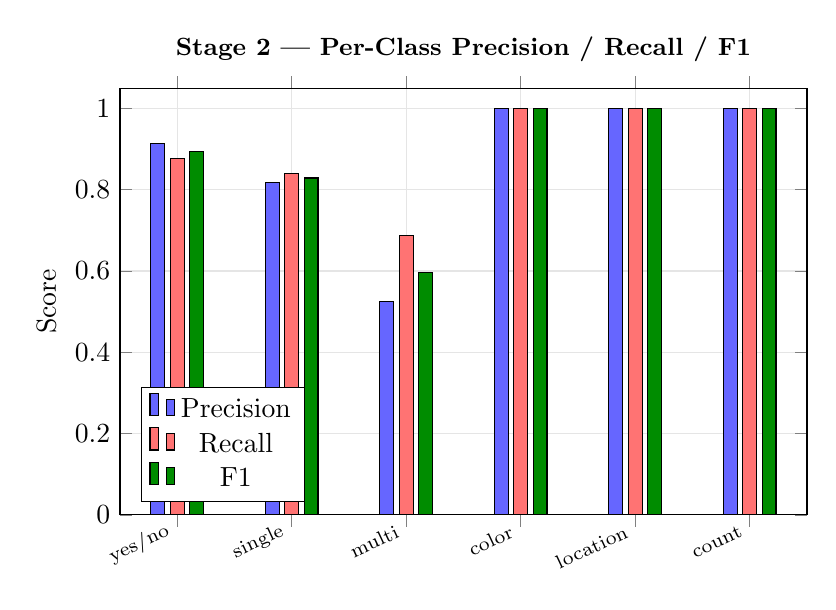
\begin{tikzpicture}
\begin{axis}[ybar, width=0.85\linewidth, height=7cm,
    title={\textbf{Stage 2 --- Per-Class Precision / Recall / F1}},
    title style={font=\small\bfseries}, ylabel={Score}, ymin=0, ymax=1.05,
    symbolic x coords={yes/no,single,multi,color,location,count}, xtick=data,
    x tick label style={rotate=25, anchor=east, font=\scriptsize},
    legend pos=south west, bar width=5pt, grid=major, grid style={gray!20}]
\addplot[fill=blue!60] coordinates {(yes/no,0.913) (single,0.818) (multi,0.526) (color,1.000) (location,0.999) (count,1.000)};
\addlegendentry{Precision}
\addplot[fill=red!55] coordinates {(yes/no,0.876) (single,0.840) (multi,0.687) (color,1.000) (location,1.000) (count,1.000)};
\addlegendentry{Recall}
\addplot[fill=green!55!black] coordinates {(yes/no,0.894) (single,0.829) (multi,0.596) (color,1.000) (location,1.000) (count,1.000)};
\addlegendentry{F1}
\end{axis}\end{tikzpicture}
\caption[Stage 2 per-class metrics]{Stage~2 per-class precision, recall, and F1
on the test set. Support: yes/no~4657, single~2618, multi~377, color~1912, location~3192, count~3199.}
\label{fig:stage2_per_class_prf}
\end{figure}
